\documentclass[11pt,a4paper]{article}
\usepackage[utf8]{inputenc}
\usepackage[spanish]{babel}	%Idioma
\usepackage{amsmath}
\usepackage{amsfonts}
\usepackage{amssymb}
\usepackage{graphicx} 	%Añadir imágenes
\usepackage{geometry}	%Ajustar márgenes
\usepackage[export]{adjustbox}[2011/08/13]
\usepackage{float}
\restylefloat{table}
\usepackage[hidelinks]{hyperref}
\usepackage{titling}
\graphicspath{{/home/nazaret/Escritorio/LaTEX}}
%\usepackage{minted}
\usepackage{multirow}
\usepackage{caption}
\usepackage{multicol}
\usepackage[shortlabels]{enumitem}
\usepackage{array}
\selectlanguage{spanish}

%Opciones de encabezado y pie de página:
\usepackage{fancyhdr}
\pagestyle{fancy}
\lhead{Nazaret Román Guerrero}
\rhead{Procesamiento Digital de Señales}
\lfoot{Grado en Ingeniería Informática}
\cfoot{}
\rfoot{\thepage}
\renewcommand{\headrulewidth}{0.4pt}
\renewcommand{\footrulewidth}{0.4pt}

%Opciones de fuente:
\usepackage[utf8]{inputenc}
\usepackage[default]{sourcesanspro}
\usepackage{sourcecodepro}
\usepackage[T1]{fontenc}

\setlength{\parindent}{15pt}
\setlength{\headheight}{15pt}
\setlength{\voffset}{10mm}

% Custom colors
\usepackage{color}
\definecolor{deepblue}{rgb}{0,0,0.5}
\definecolor{deepred}{rgb}{0.6,0,0}
\definecolor{deepgreen}{rgb}{0,0.5,0}

\usepackage{listings}
\usepackage{color}
\usepackage{graphicx}

\definecolor{dkgreen}{rgb}{0,0.6,0}
\definecolor{gray}{rgb}{0.5,0.5,0.5}
\definecolor{mauve}{rgb}{0.58,0,0.82}

\lstset{frame=tb,
  language=Matlab,
  aboveskip=3mm,
  belowskip=3mm,
  showstringspaces=false,
  columns=flexible,
  basicstyle={\small\ttfamily},
  numbers=left,
  numberstyle=\tiny\color{gray},
  keywordstyle=\color{blue},
  commentstyle=\color{dkgreen},
  stringstyle=\color{mauve},
  breaklines=true,
  breakatwhitespace=true,
  tabsize=4
}

\begin{document}
\begin{titlepage}

\begin{minipage}{\textwidth}

\centering

\includegraphics[width=0.55\textwidth]{img/logo.png}\\

\textsc{\Large Procesamiento Digital de Señales\\[0.2cm]}
\textsc{GRADO EN INGENIERÍA INFORMÁTICA}\\[1cm]

{\Huge\bfseries Práctica 3\\}
\noindent\rule[-1ex]{\textwidth}{3pt}\\[3.5ex]
{\large\bfseries Sistemas discretos. Respuesta temporal}
\end{minipage}

\vspace{1.5cm}
\begin{minipage}{\textwidth}
\centering

\textbf{Autora}\\ {Nazaret Román Guerrero}\\[2.5ex]

\includegraphics[width=0.3\textwidth]{img/etsiit.jpeg}\\[0.1cm]
\vspace{1cm}
\textsc{Escuela Técnica Superior de Ingenierías Informática y de Telecomunicación}\\
\vspace{1cm}
\textsc{Curso 2018-2019}
\end{minipage}
\end{titlepage}

\pagenumbering{gobble}
\pagenumbering{arabic}
\tableofcontents
\thispagestyle{empty}

\newpage

\section{Filtros IIR}

A pesar de no haber sido capaz de instalar Matlab y no haberlo podido usarlo para la práctica anterior (ya que dependía de un fichero que no podía subir), encontré un intérprete online que sí he podido utilizar para esta práctica.\\

El intérprete es \color{blue} \url{https://octave-online.net/}\color{black}.

\subsection{Representación gráfica del filtro IIR}

Utilizando el código proporcionado solo debemos ejecutarlo. El código está incluido bajo el nombre de \texttt{filtro\_iir.m}.

\begin{lstlisting}[frame=single]
	% Se define el array con los pulsos
   	x=[1 zeros(1,29)];
   	
   	% Se definen los coeficientes de las ecuaciones en diferencias
	a=[1 0 0.9];
	b=[0.3 0.6 0.3];
	
	% Muestra actual
	xn=[0 0 0];
	yn=[0 0 0];
	
	for n=1:length(x)
		% Los valores cambian en cada vuelta
		xn(3)=xn(2); xn(2)=xn(1); xn(1)=x(n);
		
		yn(3)=yn(2); yn(2)=yn(1); yn(1)=0.;
		
		% Se calcula el resultado de operacion de filtrado
		y(n) = -a*yn' +b*xn';
		
		% Se actualizan los valores
		yn(1)=y(n);
	end
	
	% Pintamos la grafica discreta y continua
	stem(y);
\end{lstlisting}

Se crea el array con los impulsos, se definen los coeficientes de las ecuaciones en diferencias y se calcula mediante un doble bucle. Una vez hecho, se genera la gráfica que muestra los valores discretos donde toma valor el filtro, como se puede observar en la siguiente imagen:

\begin{figure}[H]
	\centering
	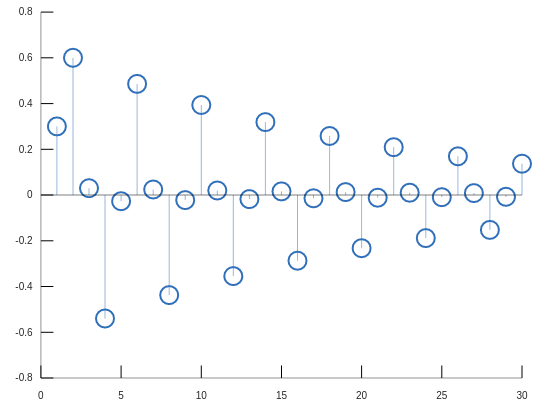
\includegraphics[scale=0.5]{img/stem1.png}
\end{figure}

Como se puede observar, el filtro hace que la señal tenga un pico al principio y vaya decreciendo (la parte positiva) y creciendo (la parte negativa) para estabilizarse en torno al valor 0.

\subsection{Función \texttt{filter} de Matlab}

Si en lugar de utilizar una función programada a mano utilizamos la función \texttt{filter} que ya viene definida en Matlab, quedaría el siguiente código (\texttt{filtro\_iir\_filter.m}):

\begin{lstlisting}[frame=single]
	% Se define el array con los pulsos
   	x=[1 zeros(1,29)];
   	
   	% Se definen los coeficientes de las ecuaciones en diferencias
	a=[1 0 0.9];
	b=[0.3 0.6 0.3];
	
	filtro = filter(b, a, x)
	
	% Pintamos la grafica discreta y continua
	stem(filtro);
\end{lstlisting}

La salida es exactamente la misma que en el caso anterior, como se puede observar:

\begin{figure}[H]
	\centering
	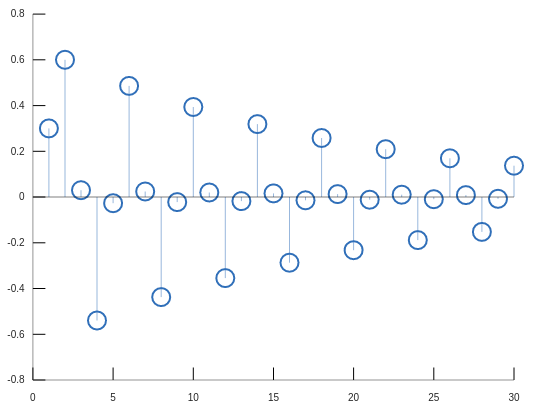
\includegraphics[scale=0.5]{img/stem-filter.png}
\end{figure}

Eso significa que el filtro implementado en el apartado anterior es correcto, ya que funciona igual que el filtro propio del lenguaje.

\subsection{Respuesta con el escalón unitario}

Ahora vamos a cambiarlo para utilizar el escalón unitario en lugar del impulso unitario como ocurría en el caso anterior. El hecho de que sea escalón significa que todos los valores mayores que 0 toman el valor 1, es decir:

\[\delta(n)=\begin{cases} 
      1, & n\geq 0\\
      0, & n< 0
   \end{cases}
\]

 mientras que en el caso de el impulso unitario solo toma el valor 1 cuando $n=0$.\\
 
Para tener el escalón unidad solo debemos cambiar la siguiente línea del código anterior (incluido como \texttt{filtro\_iir\_escalon.m}):

\begin{lstlisting}[frame=single]
	% Se define el array con los pulsos. El escalon unitario
   	x=[ones(1,30)];
\end{lstlisting}

Como es de esperar, los valores se ven aumentados. No hay valores negativos pero a pesar de ello se puede seguir observando la tendencia a estabilizarse del filtro alrededor del 0.4:

\begin{figure}[H]
	\centering
	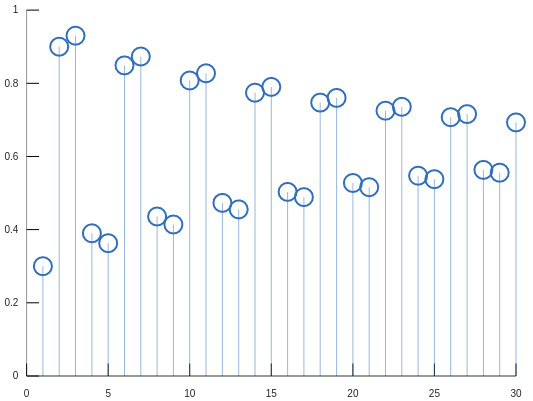
\includegraphics[scale=0.5]{img/iir-escalon.png}
\end{figure}

\subsection{¿Es estable el sistema anterior?}

Un sistema es estable si da lugar a una respuesta acotada, es decir, que no tiende a infinito. Es decir, se cumple que:

\[
	\sum_{n=0}^{\infty}\mid h(n) \mid < \infty
\]

Esto significa que el sistema del impulso unitario que hemos implementado sí es estable, ya que tiende a 0 como se puede ver claramente en la gráfica generada.

\subsection{¿Es estable el siguente sistema?}

Dada la ecuación en diferencias:

\[y(n)-2.5y(n-1)+y(n-2)=4x(n)\]

Vamos a ejecutar el código para extraer la gráfica. Usando el código anterior solo tenemos que cambiar dos líneas (fichero incluido como \texttt{filtro\_iir\_ap5.m}):

\begin{lstlisting}[frame=single]
 % Se definen los coeficientes de las ecuaciones en diferencias
a=[1 -2.5 1];
b=[4 0 0];
\end{lstlisting}

Teniendo esto en cuenta solo necesitamos ejecutar el código para ver la salida. En este caso, se puede ver claramente que el sistema no es estable, ya que la suma no está acotada.

\begin{figure}[H]
	\centering
	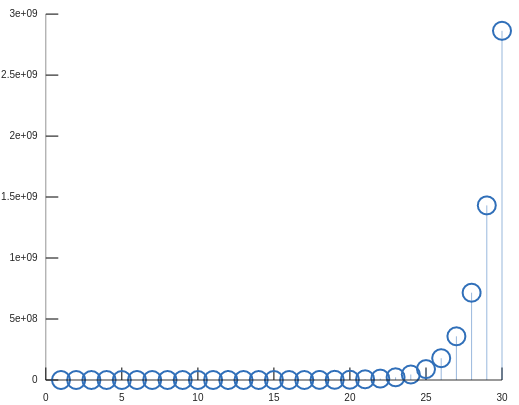
\includegraphics[scale=0.5]{img/iir-inestable.png}
\end{figure}

Se puede observar como la gráfica tiende a infinito y por tanto no es estable.
	
\newpage
	
\section{Filtros FIR}

En este caso vamos a hacer un filtro que utilice las 10 muestras anteriores para hacer una media. El código, incluido como \texttt{filtro\_fir.m}, es el siguiente:

\begin{lstlisting}[frame=single]
	% Se define el array con los pulsos
	x=[1 zeros(1,29)];

	% Coeficientes
	b = 0.1 * ones(1,10);
	a = 1;

	% Muestra actual
	xn = zeros(1,10);
	yn = zeros(1,10);

	% Se calculan los pulsos
	for n=1:length(x)
		for m=length(b):-1:2
			xn(m) = xn(m-1);
			yn(m) = yn(m-1);
		end

		xn(1)=x(n);
		yn(1)=0.;

		% Se hace la media de los 10 valores al multiplicar por b
		y(n) = b*xn';
	end

	stem(y);
\end{lstlisting}

Como se puede ver en el código, en el bucle for interno se hace la suma de las 10 muestras anteriores (inicialmente estas muestras valen 0 y todas tienen el mismo peso, 0.1, reflejado en el array \texttt{h}).\\

La salida proporcionada es la siguiente:

\begin{figure}[H]
	\centering
	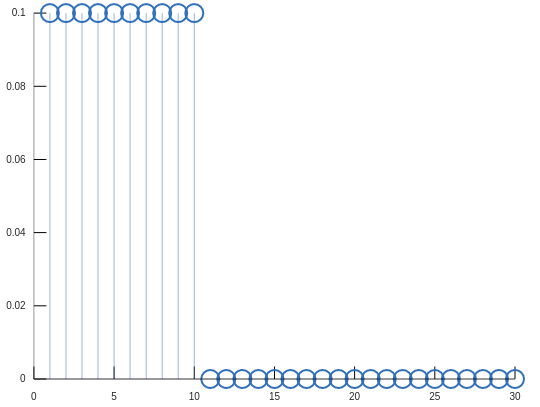
\includegraphics[scale=0.5]{img/fir-grafica.png}
\end{figure}

\subsection{Función \texttt{filter} de Matlab}

En este caso vamos a utilizar la función \texttt{filter} que hemos utilizado anteriormente, pero con un filtro FIR en respuesta al escalón unitario. El código es el siguiente (incluido con el nombre de \texttt{filtro\_fir\_escalon\_filter.m}):

\begin{lstlisting}[frame=single]
% Se define el array con los pulsos
x=[ones(1,30)];

% Coeficientes
b = 0.1 * ones(1,10);
a = 1;

filtro = filter(b, a, x)

stem(filtro)
\end{lstlisting}

Primero se crean los impulsos del escalón unitario, se define el número de muestras y el peso de cada una, se crea la memoria para acumular los valores y se aplica el filtro. Tras esto lo mostramos la gráfica.\\

\begin{figure}[H]
	\centering
	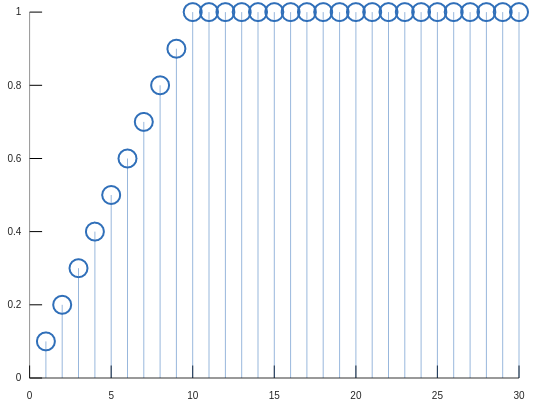
\includegraphics[scale=0.5]{img/fir-escalon-filter.png}
\end{figure}

Como se puede observar, el filtro tarda 9 muestras en estabilizarse; la 10ª muestra se estabiliza a 1 y a partir de ahí todas toman el mismo valor. Por tanto, el retardo es de 9 muestras.

\subsection{Función \texttt{conv} de Matlab}

Finalmente vamos a probar a usar la función \texttt{conv}. Solo debemos cambiar una línea del código anterior:

\begin{lstlisting}[frame=single]
filtro = conv(b, x);
\end{lstlisting}

El código está incluido bajo el nombre de \texttt{filtro\_fir\_conv.m}. Utilizando esta funcion la salida es la siguiente:

\begin{figure}[H]
	\centering
	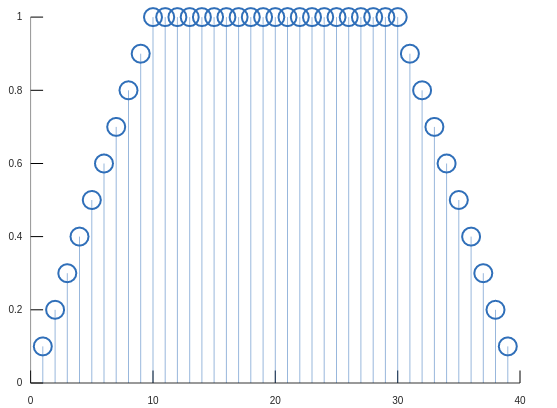
\includegraphics[scale=0.5]{img/fir-conv.png}
\end{figure}

Como podemos ver, en la convolución con 30 muestras se aplica un filtro que da lugar a una salida con 40 puntos. Esto se debe a que la convolución es una operación que multiplica (de acuerdo con la documentación oficial), por lo que los valores se ven aumentados.\\

La diferencia con la función \texttt{filter} es evidente: mientras que ésta se mantiene en el valor 1 cuando llega a él en la muestra 10, la convolución forma una subida con 10 muestras (las que se indican en el vector h), y una bajada con el mismo número de muestras. El resto de muestras se mantienen constantes entre la subida y la bajada formadas. Es decir, la diferencia principal con \texttt{filter} es que \texttt{conv} utiliza 10 muestras para realidad una bajada.

\end{document}